\documentclass[border=2mm]{standalone}
\usepackage{tikz}
\usetikzlibrary{positioning,shadows,backgrounds,shapes.geometric}
\begin{document}
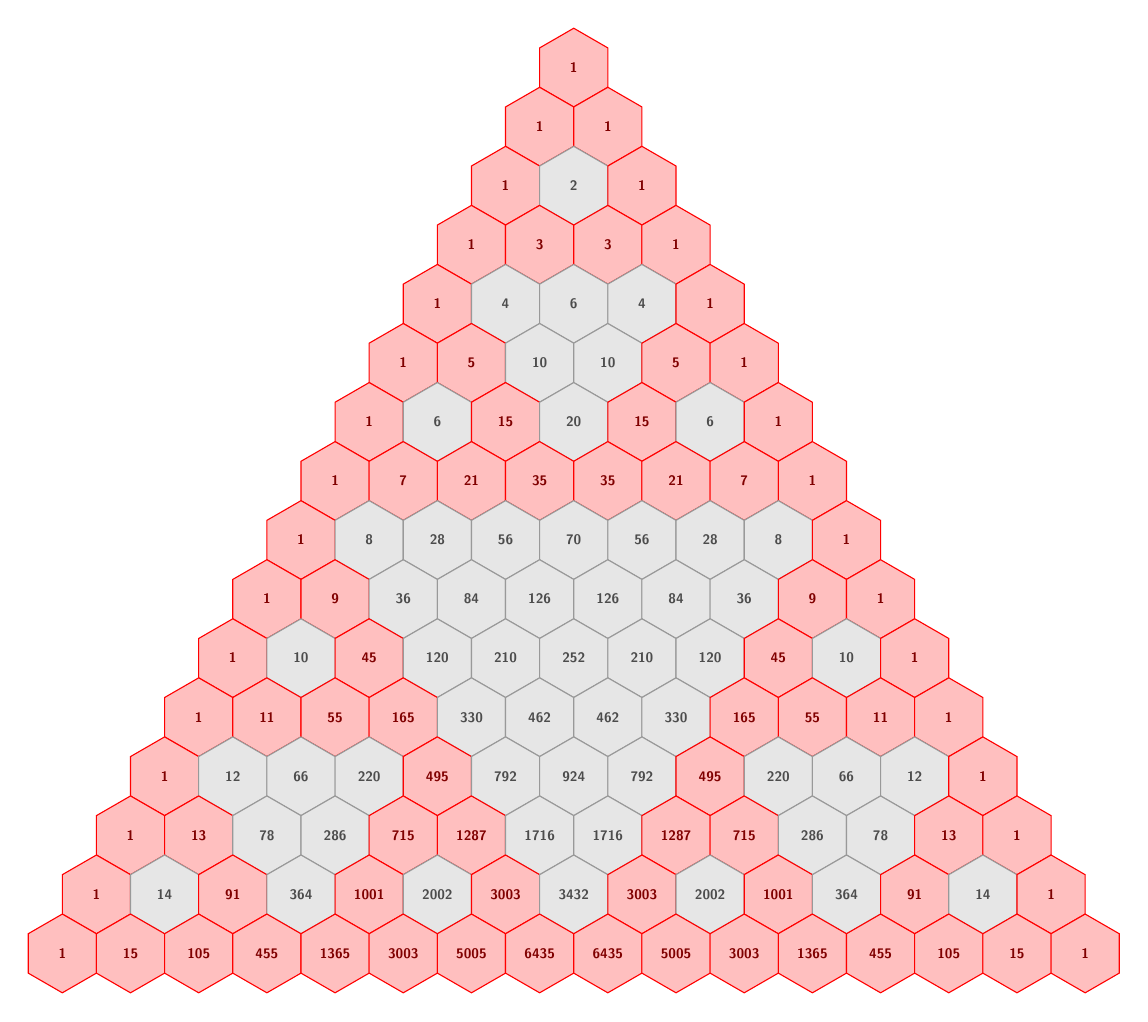
\begin{tikzpicture}[y=7.5mm,x=8.66mm]
  % some colors
  \colorlet{even}{white!60!black}
  \colorlet{odd}{red!100!black}
  % some styles
  \tikzset{
    box/.style={
      regular polygon,
      regular polygon sides=6,
      minimum size=10mm,
      inner sep=0mm,
      outer sep=0mm,
      text centered,
      font=\tiny\bfseries\sffamily,
      text=#1!50!black,
      draw=#1,
      fill=#1!25!white,fill opacity=1,
      %line width=.25mm,
      rotate=30,
    },
    link/.style={black,  shorten >=2mm, shorten <=2mm, line width=1mm},
  }
  % Pascal's triangle
  % row #0 => value is 1
  \node[box=odd] (p-0-0) at (0,0) {\rotatebox{-30}{1}};
  \foreach \row in {1,...,15} {
     % col #0 =&gt; value is 1
    \node[box=odd] (p-\row-0) at (-\row/2,-\row) {\rotatebox{-30}{1}};
    \pgfmathsetmacro{\value}{1};
    \foreach \col in {1,...,\row} {
      % iterative formula : val = precval * (row-col+1)/col
      % (+ 0.5 to bypass rounding errors)
      \pgfmathtruncatemacro{\value}{\value*((\row-\col+1)/\col)+0.5};
      \global\let\value=\value
      % position of each value
      \coordinate (pos) at (-\row/2+\col,-\row);
      % odd color for odd value and even color for even value
      \pgfmathtruncatemacro{\rest}{mod(\value,2)}
      \ifnum \rest=0
        \node[box=even] (p-\row-\col) at (pos) {\rotatebox{-30} {\value}};
      \else
        \node[box=odd] (p-\row-\col) at (pos) {\rotatebox{-30} {\value}};
      \fi      
      }
  }
\end{tikzpicture}
\end{document}